\chapter{Logistic Regression}
\lecture{10}{7 Oct.}{}

\begin{prev}
    Linear regression (\autoref{alg:linreg}) found the analytic solution
    \(\bm{w}_{\mathrm{LIN}} = \mathrm{X}^\dagger \bm{y}\) with linear regression hypotheses and squared
    error. Linear models so far answer either yes/no (perceptron, sign of the
    score) or an arbitrary real number (linear regression, the score itself).
\end{prev}

This chapter treats a third kind of question: how \emph{likely} is \(+1\)? The
answer is a probability, so the score is squashed into \([0, 1]\) by the
logistic function. The error measure is then derived rather than chosen, from
maximum likelihood, and it has no closed-form minimiser; minimising it calls for
an iterative method, gradient descent, which recasts PLA as one instance of a
general scheme.

\section{Logistic Regression Problem}\label{sec:logreg-problem}

\source{slides p.2--7}

\subsection{Heart Attack Prediction Problem (1/2)}

A new application, drawn in the noisy flow of \autoref{sec:algo-error}: from a
patient's record, predict heart disease.

\begin{center}
    \begin{adjustbox}{max width=\textwidth}
        \begin{tikzpicture}
            \node[mlbox, minimum width=4.4cm, draw=orange!85!black,
                fill=orange!8] (f) at (0,2.4)
                {unknown target\\
                 distribution \(P(y \mid \bm{x})\)\\
                 containing \(f(\bm{x})\) \(+\) noise};
            \node[mlbox, minimum width=5.2cm] (D) at (0,0)
                {training examples\\
                 \(\mathcal{D}\colon (\bm{x}_1, y_1), \dots ,
                 (\bm{x}_N, y_N)\)};
            \node[mlop, minimum width=2.4cm] (A) at (5.4,0)
                {learning\\algorithm\\\(\mathcal{A}\)\\
                 \colorbox{Purple!18}{\(\errhat\)}};
            \node[mlbox, minimum width=3.4cm] (g) at (10.2,0)
                {final hypothesis\\\(g \approx f\)};
            \node[mlbox, minimum width=3.4cm] (H) at (5.4,-2.6)
                {hypothesis set\\\(\mathcal{H}\)};
            \node[mlbox, minimum width=2.8cm, draw=blue!80!black] (e)
                at (10.2,-2.6) {error measure\\\(\err\)};
            \node[mlbox, minimum width=4.6cm] (tab) at (8.6,2.7)
                {\scriptsize
                 \begin{tabular}{@{}lr@{}}
                     age               & 40 years\\
                     gender            & male\\
                     blood pressure    & 130/85\\
                     cholesterol level & 240\\
                     weight            & 70\\
                 \end{tabular}\\[3pt]
                 \small heart disease? \textbf{yes}};
            \draw[mlarrow] (f) -- (D);
            \draw[mlarrow] (D) -- (A);
            \draw[mlarrow] (A) -- (g);
            \draw[mlarrow] (H) -- (A);
            \draw[mlarrow, draw=blue!80!black] (e) -- (g);
            \draw[mlarrow, draw=blue!80!black] (e.west)
                .. controls (7.6,-2.6) and (6.6,-1.6) .. (A.south east);
        \end{tikzpicture}
    \end{adjustbox}
\end{center}

The labels are yes/no, measured by 0/1 error, so by
\autoref{prop:mini-target} the ideal mini-target picks the more probable
label:

\begin{moral}
    Binary classification: ideal \(f(\bm{x}) = \sign \left( P(+1 \mid \bm{x})
    - \frac{1}{2} \right) \in \left\{ -1, +1 \right\}\), because of
    classification \(\err\).
\end{moral}

\subsection{Heart Attack Prediction Problem (2/2)}

Same flow, same patient, a different question:

\begin{center}
    \small
    \begin{tabular}{@{}|l|r|@{}}
        \hline
        age & 40 years\\
        gender & male\\
        blood pressure & 130/85\\
        cholesterol level & 240\\
        weight & 70\\
        \hline
    \end{tabular}\\[4pt]
    heart \textcolor{Purple}{attack}? \textbf{\textcolor{Purple}{80\% risk}}
\end{center}

A doctor would rather say `80\% risk' than `yes', since the number tells how
urgent treatment is and the yes/no answer is just the number thresholded at
\(\frac{1}{2}\).

\begin{moral}
    `Soft' binary classification: \(f(\bm{x}) = P(+1 \mid \bm{x}) \in [0,
    1]\).
\end{moral}

\subsection{Soft Binary Classification}

\begin{definition}[Soft binary classification]\label{def:soft-binary}
    \vocab{Soft binary classification} is learning the target function
    \(f(\bm{x}) = P(+1 \mid \bm{x}) \in [0, 1]\).
\end{definition}

The ideal data for it would carry the probabilities themselves; the data we
actually get carry one label drawn from each:

\begin{center}
    \begin{adjustbox}{max width=\textwidth}
        \solidrules
        \begin{tabular}{@{}l|l|l@{}}
            \toprule
            \textbf{ideal (noiseless) data} & \textbf{actual (noisy) data}
            & \textbf{actual data, as numbers}\\
            \midrule
            \(\bigl( \bm{x}_1, y_1' = 0.9 = P(+1 \mid \bm{x}_1) \bigr)\)
            & \(\bigl( \bm{x}_1, y_1 = \dmark{o} \sim P(y \mid \bm{x}_1)
            \bigr)\)
            & \(\bigl( \bm{x}_1, y_1' = 1 = \llbracket \dmark{o}
            \overset{?}{\sim} P(y \mid \bm{x}_1) \rrbracket \bigr)\)\\
            \(\bigl( \bm{x}_2, y_2' = 0.2 = P(+1 \mid \bm{x}_2) \bigr)\)
            & \(\bigl( \bm{x}_2, y_2 = \dmark{x} \sim P(y \mid \bm{x}_2)
            \bigr)\)
            & \(\bigl( \bm{x}_2, y_2' = 0 = \llbracket \dmark{o}
            \overset{?}{\sim} P(y \mid \bm{x}_2) \rrbracket \bigr)\)\\
            \qquad \(\vdots\) & \qquad \(\vdots\) & \qquad \(\vdots\)\\
            \(\bigl( \bm{x}_N, y_N' = 0.6 = P(+1 \mid \bm{x}_N) \bigr)\)
            & \(\bigl( \bm{x}_N, y_N = \dmark{x} \sim P(y \mid \bm{x}_N)
            \bigr)\)
            & \(\bigl( \bm{x}_N, y_N' = 0 = \llbracket \dmark{o}
            \overset{?}{\sim} P(y \mid \bm{x}_N) \rrbracket \bigr)\)\\
            \bottomrule
        \end{tabular}
    \end{adjustbox}
\end{center}

The last column rewrites each noisy label as a number, \(1\) if the draw came
out \(\dmark{o}\) and \(0\) otherwise: a noisy version of the ideal \(y'_n\),
whose average over many draws at \(\bm{x}_n\) would be \(P(+1 \mid
\bm{x}_n)\).

\begin{moral}
    Same data as hard binary classification, different target function.
\end{moral}

So the task is harder than it looks: we want probabilities but only ever see
0/1 outcomes.

\subsection{Logistic Hypothesis}

\begin{center}
    \small
    \begin{tabular}{@{}|l|r|@{}}
        \hline
        age & 40 years\\
        gender & male\\
        blood pressure & 130/85\\
        cholesterol level & 240\\
        \hline
    \end{tabular}
\end{center}

\begin{center}
    \begin{minipage}[c]{0.6\textwidth}
        \begin{itemize}
            \item For \(\bm{x} = (x_0, x_1, x_2, \dots , x_d)\) `features of
                patient', calculate a weighted `risk score':
                \[
                    s = \sum_{i=0}^{d} w_i x_i .
                \]
            \item Convert the score to estimated probability by logistic
                function \(\theta(s)\).
        \end{itemize}
    \end{minipage}%
    \begin{minipage}[c]{0.36\textwidth}
        \centering
        \thetacurve
    \end{minipage}
\end{center}

\begin{moral}
    Logistic hypothesis: \(h(\bm{x}) = \theta(\bm{w}^\top \bm{x})\).
\end{moral}

The score is the perceptron's and linear regression's; only the last step
differs, and it is chosen so that the output lands in \([0, 1]\).

\subsection{Logistic Function}

\begin{center}
    \thetacurve[1.2]
\end{center}

\begin{definition}[Logistic function]\label{def:logistic}
    The \vocab{logistic function} is
    \[
        \theta(s) = \frac{e^s}{1 + e^s} = \frac{1}{1 + e^{-s}} ,
    \]
    with \(\theta(-\infty) = 0\), \(\theta(0) = \frac{1}{2}\) and
    \(\theta(\infty) = 1\) --- a smooth, monotonic, \vocab{sigmoid}
    (S-shaped) function of \(s\).
\end{definition}

Two facts are used below. It is symmetric about \((0, \frac{1}{2})\):
\[
    1 - \theta(s) = \frac{e^{-s}}{1 + e^{-s}} = \frac{1}{e^s + 1} = \theta(-s) .
\]
And its derivative is \(\theta'(s) = \frac{e^{-s}}{(1 + e^{-s})^2} =
\theta(s)\, \theta(-s) > 0\).

\begin{moral}
    Logistic regression: use
    \[
        h(\bm{x}) = \frac{1}{1 + \exp(-\bm{w}^\top \bm{x})}
    \]
    to approximate target function \(f(\bm{x}) = P(+1 \mid \bm{x})\).
\end{moral}

\begin{exercise}[Fun Time: Logistic Regression and Binary Classification]
    Consider any logistic hypothesis \(h(\bm{x}) = \frac{1}{1 + \exp(-\bm{w}^\top
    \bm{x})}\) that approximates \(P(y \mid \bm{x})\). `Convert' \(h(\bm{x})\)
    to a binary classification prediction by taking \(\sign \left( h(\bm{x}) -
    \frac{1}{2} \right)\). What is the equivalent formula for the binary
    classification prediction?
    \begin{enumerate}[(1)]
        \item \(\sign \left( \bm{w}^\top \bm{x} - \frac{1}{2} \right)\);
        \item \(\sign \left( \bm{w}^\top \bm{x} \right)\);
        \item \(\sign \left( \bm{w}^\top \bm{x} + \frac{1}{2} \right)\);
        \item none of the above.
    \end{enumerate}
\end{exercise}

\begin{proof}[Reference Answer]
    (2). When \(\bm{w}^\top \bm{x} = 0\), \(h(\bm{x})\) is exactly
    \(\frac{1}{2}\). So thresholding \(h(\bm{x})\) at \(\frac{1}{2}\) is the
    same as thresholding \(\bm{w}^\top \bm{x}\) at \(0\), since \(\theta\) is
    increasing. A logistic hypothesis thus carries a perceptron inside it, and
    soft classification refines the hard one.
\end{proof}

\section{Logistic Regression Error}\label{sec:logreg-error}

\source{slides p.8--12}

The hypothesis set is fixed; what is missing is the error measure that
\(\mathcal{A}\) minimises.

\subsection{Three Linear Models}

All three models compute the same linear scoring function \(s = \bm{w}^\top
\bm{x}\) and differ in what they do with it:

\begin{center}
    \begin{adjustbox}{max width=\textwidth}
        \solidrules
        \begin{tabular}{@{}c|c|c@{}}
            \toprule
            \textbf{linear classification} & \textbf{linear regression}
            & \textbf{logistic regression}\\
            \(h(\bm{x}) = \sign(s)\) & \(h(\bm{x}) = s\)
            & \(h(\bm{x}) = \theta(s)\)\\
            \midrule
            \scoreunit{sign} & \scoreunit{id} & \scoreunit{theta}\\[4pt]
            plausible \(\err\) \(=\) 0/1 & friendly \(\err\) \(=\) squared
            & \textcolor{orange!85!black}{\(\err = {}\)?}\\
            \textcolor{blue!80!black}{(small flipping noise)}
            & \textcolor{blue!80!black}{(easy to minimize)} & \\
            \bottomrule
        \end{tabular}
    \end{adjustbox}
\end{center}

The first two error measures were justified in \autoref{def:errhat}. Neither
fits the third model: its output is a probability and its labels are
\(\pm 1\), so `how far is \(0.8\) from \(+1\)' needs a principled answer.

\begin{question}
    How to define \(\Ein(\bm{w})\) for logistic regression?
\end{question}

\subsection{Likelihood}

\[
    \text{target function } f(\bm{x}) = P(+1 \mid \bm{x})
    \quad \Longleftrightarrow \quad
    P(y \mid \bm{x}) = \begin{cases}
        f(\bm{x}) & \text{for } y = +1\\
        1 - f(\bm{x}) & \text{for } y = -1
    \end{cases}
\]

Consider \(\mathcal{D} = \left\{ (\bm{x}_1, \dmark{o}), (\bm{x}_2, \dmark{x}),
\dots , (\bm{x}_N, \dmark{x}) \right\}\). Each example arose by drawing
\(\bm{x}_n \sim P(\bm{x})\) and then \(y_n \sim P(y \mid \bm{x}_n)\),
independently, so:

\begin{center}
    \solidrules
    \begin{tabular}{@{}l|l@{}}
        \toprule
        \textbf{probability that \(f\) generates \(\mathcal{D}\)}
        & \textbf{likelihood that \(h\) generates \(\mathcal{D}\)}\\
        \midrule
        \(P(\bm{x}_1) P(\dmark{o} \mid \bm{x}_1) = P(\bm{x}_1) f(\bm{x}_1)
        \times{}\)
        & \(P(\bm{x}_1) h(\bm{x}_1) \times{}\)\\
        \(P(\bm{x}_2) P(\dmark{x} \mid \bm{x}_2) = P(\bm{x}_2) \bigl( 1 -
        f(\bm{x}_2) \bigr) \times{}\)
        & \(P(\bm{x}_2) \bigl( 1 - h(\bm{x}_2) \bigr) \times{}\)\\
        \(\dots\) & \(\dots\)\\
        \(P(\bm{x}_N) P(\dmark{x} \mid \bm{x}_N) = P(\bm{x}_N) \bigl( 1 -
        f(\bm{x}_N) \bigr)\)
        &\(P(\bm{x}_N) \bigl( 1 - h(\bm{x}_N) \bigr)\)\\
        \bottomrule
    \end{tabular}
\end{center}

The right column is the same computation with \(h\) pretending to be \(f\); a
probability of observed data, viewed as a function of the hypothesis, is
called its \vocab{likelihood}.

\begin{itemize}
    \item if \(h \approx f\), then likelihood(\(h\)) \(\approx\) probability
        using \(f\);
    \item probability using \(f\) usually \textbf{large}.
\end{itemize}

The second point is because \(\mathcal{D}\) really was generated by \(f\): the
sample we got is a typical one under \(f\), not one of its rare outcomes. So a
hypothesis under which \(\mathcal{D}\) looks unlikely is unlikely to be close
to \(f\).

\subsection{Likelihood of Logistic Hypothesis}

\begin{moral}
    likelihood(\(h\)) \(\approx\) (probability using \(f\)) \(\approx\) large
    \quad \(\Longrightarrow\) \quad
    \(\displaystyle g = \argmax_h \; \text{likelihood}(h)\).
\end{moral}

This is the principle of \vocab{maximum likelihood}. For logistic hypotheses
it simplifies.

\begin{center}
    \begin{minipage}[c]{0.55\textwidth}
        When logistic: \(h(\bm{x}) = \theta(\bm{w}^\top \bm{x})\),
        \[
            1 - h(\bm{x}) = h(-\bm{x}) ,
        \]
        by the symmetry \(1 - \theta(s) = \theta(-s)\) of
        \autoref{def:logistic}, with \(s = \bm{w}^\top \bm{x}\).
    \end{minipage}%
    \begin{minipage}[c]{0.4\textwidth}
        \centering
        \thetacurve
    \end{minipage}
\end{center}

Substituting into the likelihood,
\begin{align*}
    \text{likelihood}(h)
    &= P(\bm{x}_1) h(\bm{x}_1) \times P(\bm{x}_2) \bigl( 1 - h(\bm{x}_2)
    \bigr) \times \dots P(\bm{x}_N) \bigl( 1 - h(\bm{x}_N) \bigr)\\
    &= P(\bm{x}_1) h(+\bm{x}_1) \times P(\bm{x}_2) h(-\bm{x}_2) \times
    \dots P(\bm{x}_N) h(-\bm{x}_N) .
\end{align*}
The sign in front of each \(\bm{x}_n\) is its label \(y_n\), and the factors
\(P(\bm{x}_n)\) are the same for every \(h\), so they do not affect the
\(\argmax\):

\begin{moral}
    \(\displaystyle \text{likelihood(logistic } h) \propto \prod_{n=1}^N
    h(y_n \bm{x}_n)\).
\end{moral}

\subsection{Cross-Entropy Error}

Now turn the maximisation into a minimisation of an average, one step at a
time:
\begin{align*}
    &\max_h \; \text{likelihood(logistic } h) \propto \prod_{n=1}^N h(y_n
    \bm{x}_n)\\
    \iff{} &\max_{\bm{w}} \; \text{likelihood}(\bm{w}) \propto \prod_{n=1}^N
    \theta \left( y_n \bm{w}^\top \bm{x}_n \right)\\
    \iff{} &\max_{\bm{w}} \; \ln \prod_{n=1}^N \theta \left( y_n \bm{w}^\top
    \bm{x}_n \right)\\
    \iff{} &\min_{\bm{w}} \; \frac{1}{N} \sum_{n=1}^N - \ln \theta \left( y_n
    \bm{w}^\top \bm{x}_n \right) .
\end{align*}
The first line becomes the second because a logistic \(h\) \emph{is} its
\(\bm{w}\); the logarithm is increasing, so it keeps the maximiser while
turning the product into a sum; and negating and dividing by \(N\) turns the
maximum of the sum into the minimum of an average. With \(\theta(s) = \frac{1}{1
+ \exp(-s)}\), \(-\ln \theta(s) = \ln(1 + \exp(-s))\), hence
\[
    \min_{\bm{w}} \frac{1}{N} \sum_{n=1}^N \ln \left( 1 + \exp(-y_n
    \bm{w}^\top \bm{x}_n) \right)
    \quad \Longrightarrow \quad
    \min_{\bm{w}} \underbrace{\frac{1}{N} \sum_{n=1}^N \err(\bm{w}, \bm{x}_n,
    y_n)}_{\Ein(\bm{w})} .
\]

\begin{definition}[Cross-entropy error]\label{def:ce-err}
    The pointwise error
    \begin{equation}\label{eq:ce-err}
        \err(\bm{w}, \bm{x}, y) = \ln \left( 1 + \exp(-y \bm{w}^\top \bm{x})
        \right)
    \end{equation}
    is called the \vocab{cross-entropy error}.
\end{definition}

\begin{moral}
    \(\err(\bm{w}, \bm{x}, y) = \ln \left( 1 + \exp(-y \bm{w}^\top \bm{x})
    \right)\): cross-entropy error.
\end{moral}

The name: write \(y' = \llbracket y = +1 \rrbracket\) and \(p = h(\bm{x})\).
Then \(-\bigl( y' \ln p + (1 - y') \ln(1 - p) \bigr)\), the cross-entropy
between the observed label distribution \((y', 1 - y')\) and the predicted one
\((p, 1 - p)\), equals \(-\ln \theta(y \bm{w}^\top \bm{x})\), which is
\eqref{eq:ce-err}. Up to the factor \(\log_2 e\), \eqref{eq:ce-err} is also the
third upper bound of the last Fun Time of \autoref{sec:linreg-cls}.

\begin{exercise}[Fun Time]
    The four statements below help us understand more about the cross-entropy
    error \(\err(\bm{w}, \bm{x}, y) = \ln \left( 1 + \exp(-y \bm{w}^\top
    \bm{x}) \right)\). Consider \(\bm{w}^\top \bm{x} \neq 0\). Which statement
    is not true?
    \begin{enumerate}[(1)]
        \item For any \(\bm{w}\), \(\bm{x}\), and \(y\), \(\err(\bm{w}, \bm{x},
            y) > 0\).
        \item For any \(\bm{w}\), \(\bm{x}\), and \(y\), \(\err(\bm{w}, \bm{x},
            y) < 1126\).
        \item When \(y = \sign(\bm{w}^\top \bm{x})\), \(\err(\bm{w}, \bm{x}, y)
            < \ln 2\).
        \item When \(y \neq \sign(\bm{w}^\top \bm{x})\), \(\err(\bm{w},
            \bm{x}, y) \ge \ln 2\).
    \end{enumerate}
\end{exercise}

\begin{proof}[Reference Answer]
    (2). 1126, really? :-) You are highly encouraged to plot the curve of
    \(\err\) with respect to some fixed \(y\) and some varying score \(s =
    \bm{w}^\top \bm{x}\) to know more about the error measure. After plotting,
    it is easy to see that \(\err\) is not bounded above, and the other three
    choices are correct.
    \begin{center}
        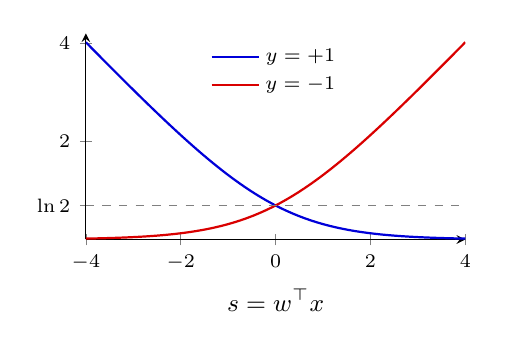
\begin{tikzpicture}
            \begin{axis}[
                width=6.4cm, height=4.2cm,
                xmin=-4, xmax=4, ymin=0, ymax=4.2,
                axis lines=left, xtick={-4,-2,0,2,4}, ytick={0.693,2,4},
                yticklabels={\(\ln 2\), \(2\), \(4\)},
                tick label style={font=\scriptsize},
                xlabel={\(s = \bm{w}^\top \bm{x}\)}, label style={font=\small},
                legend style={font=\scriptsize, draw=none, fill=none,
                    at={(0.5,0.98)}, anchor=north}]
                \addplot[blue!85!black, thick, domain=-4:4, samples=60]
                    {ln(1 + exp(-x))};
                \addplot[red!85!black, thick, domain=-4:4, samples=60]
                    {ln(1 + exp(x))};
                \addplot[black!50, dashed, domain=-4:4] {ln(2)};
                \legend{\(y = +1\), \(y = -1\)}
            \end{axis}
        \end{tikzpicture}
    \end{center}
    Each curve is positive, decreases (for \(y = +1\)) or increases (for \(y =
    -1\)) through \(\ln 2\) at \(s = 0\), and grows like \(\abs{s}\) on the
    wrong side, which settles (1), (3), (4) and refutes (2).
\end{proof}

\section{Gradient of Logistic Regression Error}\label{sec:logreg-grad}

\source{slides p.13--17}

With \(\Ein\) defined, the remaining task is the one that linear regression
solved in \autoref{sec:linreg-algo}: minimise it.

\subsection{Minimizing \texorpdfstring{\(\Ein(\bm{w})\)}{Ein(w)}}

\[
    \min_{\bm{w}} \; \Ein(\bm{w}) = \frac{1}{N} \sum_{n=1}^N \ln \left( 1 +
    \exp(-y_n \bm{w}^\top \bm{x}_n) \right)
\]

\begin{center}
    \begin{minipage}[c]{0.3\textwidth}
        \centering
        \einbowl{\(\bm{w}\)}
    \end{minipage}%
    \begin{minipage}[c]{0.66\textwidth}
        \begin{itemize}
            \item \(\Ein(\bm{w})\): continuous, differentiable,
                twice-differentiable, \textbf{convex};
            \item how to minimize? locate \textbf{valley}: want \(\nabla
                \Ein(\bm{w}) = \bm{0}\).
        \end{itemize}
    \end{minipage}
\end{center}

Convexity holds term by term: \(\ln(1 + e^{-t})\) has second derivative
\(\theta(t) \theta(-t) > 0\) in \(t\), and composing a convex function of one
variable with the linear map \(\bm{w} \mapsto y_n \bm{w}^\top \bm{x}_n\) keeps
it convex. So, as in \autoref{sec:linreg-algo}, a zero gradient means a global
minimum.

\begin{moral}
    First: derive \(\nabla \Ein(\bm{w})\).
\end{moral}

\subsection{The Gradient \texorpdfstring{\(\nabla \Ein(\bm{w})\)}{of Ein}}

Name the two nested pieces of each term, \(\textcolor{blue}{\bigcirc} =
-y_n \bm{w}^\top \bm{x}_n\) and \(\textcolor{red}{\square} = 1 +
\exp(\textcolor{blue}{\bigcirc})\):
\[
    \Ein(\bm{w}) = \frac{1}{N} \sum_{n=1}^N \ln \Bigl(
    \underbrace{1 + \exp(\overbrace{-y_n \bm{w}^\top
    \bm{x}_n}^{\textcolor{blue}{\bigcirc}})}_{\textcolor{red}{\square}}
    \Bigr) .
\]
The chain rule, one factor per layer:
\begin{align*}
    \frac{\partial \Ein(\bm{w})}{\partial w_i}
    &= \frac{1}{N} \sum_{n=1}^N
    \left( \frac{\partial \ln(\textcolor{red}{\square})}{\partial
    \textcolor{red}{\square}} \right)
    \left( \frac{\partial (1 + \exp(\textcolor{blue}{\bigcirc}))}{\partial
    \textcolor{blue}{\bigcirc}} \right)
    \left( \frac{\partial (-y_n \bm{w}^\top \bm{x}_n)}{\partial w_i}
    \right)\\
    &= \frac{1}{N} \sum_{n=1}^N
    \left( \frac{1}{\textcolor{red}{\square}} \right)
    \left( \exp(\textcolor{blue}{\bigcirc}) \right)
    \left( -y_n x_{n,i} \right)\\
    &= \frac{1}{N} \sum_{n=1}^N
    \left( \frac{\exp(\textcolor{blue}{\bigcirc})}{1 +
    \exp(\textcolor{blue}{\bigcirc})} \right)
    \left( -y_n x_{n,i} \right)
    = \frac{1}{N} \sum_{n=1}^N \theta(\textcolor{blue}{\bigcirc})
    \left( -y_n x_{n,i} \right) ,
\end{align*}
the last step by the first form of \(\theta\) in \autoref{def:logistic}.
Collecting the \(d + 1\) coordinates:

\begin{moral}
    \begin{equation}\label{eq:lr-grad}
        \nabla \Ein(\bm{w}) = \frac{1}{N} \sum_{n=1}^N \theta \left( -y_n
        \bm{w}^\top \bm{x}_n \right) \left( -y_n \bm{x}_n \right) .
    \end{equation}
\end{moral}

\subsection{Minimizing \texorpdfstring{\(\Ein(\bm{w})\)}{Ein(w)}, Again}

\begin{align*}
    \min_{\bm{w}} \; \Ein(\bm{w}) &= \frac{1}{N} \sum_{n=1}^N \ln \left( 1 +
    \exp(-y_n \bm{w}^\top \bm{x}_n) \right)\\
    \text{want } \nabla \Ein(\bm{w}) &= \frac{1}{N} \sum_{n=1}^N \theta \left(
    -y_n \bm{w}^\top \bm{x}_n \right) \left( -y_n \bm{x}_n \right) =
    \bm{0} .
\end{align*}

\begin{center}
    \begin{minipage}[c]{0.3\textwidth}
        \centering
        \einbowl{\(\bm{w}\)}
    \end{minipage}%
    \begin{minipage}[c]{0.66\textwidth}
        \eqref{eq:lr-grad} is a \textbf{scaled \(\theta\)-weighted sum of
        \(-y_n \bm{x}_n\)}:
        \begin{itemize}
            \item all \(\theta(\cdot) = 0\): only if \(y_n \bm{w}^\top \bm{x}_n
                \gg 0\) --- linear separable \(\mathcal{D}\);
            \item weighted sum \(= \bm{0}\): non-linear equation of \(\bm{w}\).
        \end{itemize}
    \end{minipage}
\end{center}

The weights \(\theta(-y_n \bm{w}^\top \bm{x}_n)\) are never exactly zero, so
the first case is only approached, as \(\norm{\bm{w}} \to \infty\) along a
direction that separates \(\mathcal{D}\); for separable data \(\Ein\) has no
finite minimiser at all. In the second case \(\bm{w}\) sits inside \(\theta\),
so unlike the normal equations of \autoref{sec:linreg-algo} this is not a linear
system.

\begin{moral}
    Closed-form solution? No :-(
\end{moral}

\subsection{PLA Revisited: Iterative Optimization}

Without a formula, we need a way to walk towards the valley. PLA already walks:
it starts from some \(\bm{w}_0\) (say, \(\bm{0}\)) and `corrects' its mistakes
on \(\mathcal{D}\). In the form of \autoref{alg:pla}, for \(t = 0, 1, \dots\):

\begin{enumerate}
    \item find a mistake of \(\bm{w}_t\) called \((\bm{x}_{n(t)}, y_{n(t)})\),
        \[
            \sign \left( \bm{w}_t^\top \bm{x}_{n(t)} \right) \neq y_{n(t)} ;
        \]
    \item (try to) correct the mistake by
        \[
            \bm{w}_{t+1} \gets \bm{w}_t + y_{n(t)} \bm{x}_{n(t)} ;
        \]
\end{enumerate}
when stop, return last \(\bm{w}\) as \(g\).

The two steps merge into one: (equivalently) pick some \(n\), and update
\(\bm{w}_t\) by
\[
    \bm{w}_{t+1} \gets \bm{w}_t + \llbracket \sign \left( \bm{w}_t^\top
    \bm{x}_n \right) \neq y_n \rrbracket \, y_n \bm{x}_n ,
\]
which moves only when \(n\) is a mistake. Read it as a step size times a
direction:
\[
    \bm{w}_{t+1} \gets \bm{w}_t + \underbrace{1}_{\eta} \cdot
    \underbrace{\left( \llbracket \sign \left( \bm{w}_t^\top \bm{x}_n
    \right) \neq y_n \rrbracket \cdot y_n \bm{x}_n \right)}_{\bm{v}} ;
\]
when stop, return last \(\bm{w}\) as \(g\).

\begin{moral}
    Choice of \((\eta, \bm{v})\) and stopping condition defines
    \textcolor{orange!85!black}{iterative optimization approach}.
\end{moral}

\begin{exercise}[Fun Time]
    Consider the gradient \(\nabla \Ein(\bm{w}) = \frac{1}{N} \sum_{n=1}^N
    \theta \left( -y_n \bm{w}^\top \bm{x}_n \right) \left( -y_n \bm{x}_n
    \right)\). That is, each example \((\bm{x}_n, y_n)\) contributes to the
    gradient by an amount of \(\theta \left( -y_n \bm{w}^\top \bm{x}_n
    \right)\). For any given \(\bm{w}\), which example contributes the most
    amount to the gradient?
    \begin{enumerate}[(1)]
        \item the example with the smallest \(y_n \bm{w}^\top \bm{x}_n\)
            value;
        \item the example with the largest \(y_n \bm{w}^\top \bm{x}_n\) value;
        \item the example with the smallest \(\bm{w}^\top \bm{x}_n\) value;
        \item the example with the largest \(\bm{w}^\top \bm{x}_n\) value.
    \end{enumerate}
\end{exercise}

\begin{proof}[Reference Answer]
    (1). Using the fact that \(\theta\) is a monotonic function, we see that
    the example with the smallest \(y_n \bm{w}^\top \bm{x}_n\) value
    contributes to the gradient the most. That is the example most badly
    misclassified --- a soft version of PLA's attention to mistakes.
\end{proof}

\section{Gradient Descent}\label{sec:gd}

\source{slides p.18--24}

PLA's \(\bm{v}\) comes from a mistake; for a smooth \(\Ein\) we can do better
and let the slope pick it.

\subsection{Iterative Optimization}

For \(t = 0, 1, \dots\)
\[
    \bm{w}_{t+1} \gets \bm{w}_t + \eta \bm{v} ;
\]
when stop, return last \(\bm{w}\) as \(g\).

\begin{center}
    \begin{minipage}[c]{0.62\textwidth}
        \begin{itemize}
            \item PLA: \(\bm{v}\) comes from mistake correction.
            \item Smooth \(\Ein(\bm{w})\) for logistic regression: choose
                \(\bm{v}\) to get the ball roll `\textbf{downhill}'?
            \begin{itemize}
                \item direction \(\bm{v}\): (assumed) of unit length;
                \item step size \(\eta\): (assumed) positive.
            \end{itemize}
        \end{itemize}
    \end{minipage}%
    \begin{minipage}[c]{0.34\textwidth}
        \centering
        \begin{tikzpicture}
            \draw[thin] (0,2.4) -- (0,0) -- (2.4,0);
            \node[rotate=90, font=\scriptsize] at (-0.25,1.2)
                {In-sample Error, \(\Ein\)};
            \node[font=\scriptsize, below] at (1.5,0) {Weights, \(\bm{w}\)};
            \draw[gdcurve] plot[domain=0.1:4.0, samples=60]
                ({0.55*\x}, {0.55*(0.75*(\x - 2.3)^2 + 0.2)});
            \fill (0.08,2.09) circle (2pt);
            \draw[-{Stealth[length=1.6mm]}, semithick] (0.12,1.98)
                -- (0.27,1.50);
        \end{tikzpicture}
    \end{minipage}
\end{center}

Fixing \(\norm{\bm{v}} = 1\) separates the two decisions: \(\bm{v}\) says where
to go, \(\eta\) how far.

\begin{moral}
    A greedy approach for some given \(\eta > 0\):
    \(\displaystyle \min_{\norm{\bm{v}} = 1} \Ein(\underbrace{\bm{w}_t + \eta
    \bm{v}}_{\bm{w}_{t+1}})\).
\end{moral}

\subsection{Linear Approximation}

A greedy approach for some given \(\eta > 0\):
\[
    \min_{\norm{\bm{v}} = 1} \; \Ein(\bm{w}_t + \eta \bm{v}) .
\]
\begin{itemize}
    \item Still non-linear optimization, now \textbf{with constraints} --- not
        any easier than \(\min_{\bm{w}} \Ein(\bm{w})\).
    \item Local approximation by linear formula makes problem easier:
        \[
            \Ein(\bm{w}_t + \eta \bm{v}) \approx \Ein(\bm{w}_t) + \eta
            \bm{v}^\top \nabla \Ein(\bm{w}_t)
        \]
        if \(\eta\) really small (Taylor expansion).
\end{itemize}

The approximation is the first-order Taylor expansion of \(\Ein\) at
\(\bm{w}_t\); its error is \(O(\eta^2)\), negligible against the linear term
when \(\eta\) is small and \(\nabla \Ein(\bm{w}_t) \neq \bm{0}\).

\begin{moral}
    An \textcolor{orange!85!black}{approximate} greedy approach for some given
    \textcolor{orange!85!black}{small} \(\eta\):
    \[
        \min_{\norm{\bm{v}} = 1} \;
        \underbrace{\Ein(\bm{w}_t)}_{\text{known}} +
        \underbrace{\eta}_{\text{given positive}}
        \bm{v}^\top \underbrace{\nabla \Ein(\bm{w}_t)}_{\text{known}} .
    \]
\end{moral}

\subsection{Gradient Descent}

In the approximate problem the first term is a constant and \(\eta > 0\), so
only \(\bm{v}^\top \nabla \Ein(\bm{w}_t)\) is to be minimised over unit
vectors.

\begin{itemize}
    \item Optimal \(\bm{v}\): opposite direction of \(\nabla \Ein(\bm{w}_t)\),
        \[
            \bm{v} = - \frac{\nabla \Ein(\bm{w}_t)}{\norm{\nabla
            \Ein(\bm{w}_t)}} .
        \]
    \item Gradient descent: for \textbf{small} \(\eta\),
        \(\displaystyle \bm{w}_{t+1} \gets \bm{w}_t - \eta \frac{\nabla
        \Ein(\bm{w}_t)}{\norm{\nabla \Ein(\bm{w}_t)}}\).
\end{itemize}

The optimal \(\bm{v}\) follows from Cauchy--Schwarz (as in
\autoref{rmk:cauchy}):
\[
    \bm{v}^\top \nabla \Ein(\bm{w}_t) \ge -\norm{\bm{v}} \norm{\nabla
    \Ein(\bm{w}_t)} = -\norm{\nabla \Ein(\bm{w}_t)} ,
\]
with equality exactly when \(\bm{v}\) points opposite to the gradient.

\begin{definition}[Gradient descent]\label{def:gd}
    \vocab{Gradient descent} is the iterative optimisation that repeatedly
    steps against the gradient, \(\bm{w}_{t+1} \gets \bm{w}_t - \eta \nabla
    \Ein(\bm{w}_t) / \norm{\nabla \Ein(\bm{w}_t)}\).
\end{definition}

\begin{moral}
    Gradient descent: a simple \& popular optimization tool.
\end{moral}

\subsection{Choice of \texorpdfstring{\(\eta\)}{eta}}

The derivation assumed \(\eta\) small, but how small? Three runs on a
one-dimensional \(\Ein\) of my own (a parabola) show what goes wrong; every
iterate drawn is computed, not sketched.

\begin{center}
    \begin{adjustbox}{max width=\textwidth}
        \begin{tikzpicture}[font=\scriptsize]
            % too small: constant step 0.13 along -sign of the slope
            \begin{scope}
                \node[font=\small\bfseries] at (1.2,2.75) {too small};
                \draw[thin] (0,2.4) -- (0,0) -- (2.4,0);
                \node[rotate=90] at (-0.25,1.2) {In-sample Error, \(\Ein\)};
                \node[below] at (1.5,0) {Weights, \(\bm{w}\)};
                \draw[gdcurve] plot[domain=0.1:4.0, samples=60]
                    ({0.55*\x}, {0.55*(0.75*(\x - 2.3)^2 + 0.2)});
                \draw[gdpath] (0.08,2.02) -| (0.15,1.79) -| (0.23,1.58)
                    -| (0.3,1.39) -| (0.37,1.21) -| (0.44,1.04) -| (0.51,0.88)
                    -| (0.58,0.74) -| (0.65,0.62) -| (0.73,0.51) -| (0.8,0.41)
                    -| (0.87,0.32) -| (0.94,0.25) -| (1.01,0.2) -| (1.08,0.15);
                \node[font=\small\bfseries] at (1.2,-0.65) {too slow :-(};
            \end{scope}
            % too large: each step lands past the bottom of a narrow valley
            \begin{scope}[xshift=3.4cm]
                \node[font=\small\bfseries] at (1.2,2.75) {too large};
                \draw[thin] (0,2.4) -- (0,0) -- (2.4,0);
                \node[rotate=90] at (-0.25,1.2) {In-sample Error, \(\Ein\)};
                \node[below] at (1.5,0) {Weights, \(\bm{w}\)};
                \draw[gdcurve] plot[domain=0.8:3.2, samples=60]
                    ({0.55*\x}, {0.55*(2.6*(\x - 2)^2 + 0.25)});
                \draw[gdpath] (0.47,2.03) -- (1.64,1.49) -- (0.65,1.11)
                    -- (1.48,0.83) -- (0.78,0.63) -- (1.37,0.49)
                    -- (0.87,0.39) -- (1.3,0.32);
                \node[font=\small\bfseries] at (1.2,-0.65)
                    {too unstable :-(};
            \end{scope}
            % just right: step proportional to the slope
            \begin{scope}[xshift=6.8cm]
                \node[font=\small\bfseries] at (1.2,2.75) {just right};
                \draw[thin] (0,2.4) -- (0,0) -- (2.4,0);
                \node[rotate=90] at (-0.25,1.2) {In-sample Error, \(\Ein\)};
                \node[below] at (1.5,0) {Weights, \(\bm{w}\)};
                \draw[gdcurve] plot[domain=0.1:4.0, samples=60]
                    ({0.55*\x}, {0.55*(0.75*(\x - 2.3)^2 + 0.2)});
                \draw[gdpath] (0.08,2.02) -| (0.83,0.37) -| (1.1,0.15)
                    -| (1.21,0.11) -| (1.24,0.11) -| (1.26,0.11);
                \node[anchor=west] at (0.85,2.15) {large \(\eta\)};
                \node[anchor=west, inner sep=1pt] at (0.9,0.85) {small \(\eta\)};
                \node[font=\small\bfseries, text=orange!85!black]
                    at (1.2,-0.65) {use changing \(\eta\)};
            \end{scope}
        \end{tikzpicture}
    \end{adjustbox}
\end{center}

Left, a fixed small step: every move goes the right way, but by the same
small amount however steep the slope, so progress is slow. Middle, steps too
long for the curvature: each one overshoots the bottom and lands on the other
wall, and the iterates bounce across the valley. Right, the step shrinks as
the slope flattens: large far away, small near the bottom.

\begin{moral}
    \(\eta\) better be monotonic of \(\norm{\nabla \Ein(\bm{w}_t)}\).
\end{moral}

\subsection{Simple Heuristic for Changing \texorpdfstring{\(\eta\)}{eta}}

\begin{itemize}
    \item If \textcolor{red}{\(\eta\)} \(\propto \norm{\nabla
        \Ein(\bm{w}_t)}\) by ratio \textcolor{Purple}{\(\eta\)}, i.e.\
        \(\textcolor{red}{\eta} = \textcolor{Purple}{\eta} \norm{\nabla
        \Ein(\bm{w}_t)}\),
        \[
            \bm{w}_{t+1} \gets \bm{w}_t - \textcolor{red}{\eta} \frac{\nabla
            \Ein(\bm{w}_t)}{\norm{\nabla \Ein(\bm{w}_t)}}
            = \bm{w}_t - \textcolor{Purple}{\eta} \nabla \Ein(\bm{w}_t) .
        \]
    \item Call \textcolor{Purple}{\(\eta\)} the \vocab{fixed learning rate}.
\end{itemize}

The normalisation and the proportional step cancel, so the update is simply
the raw gradient times a constant. The step length still varies, since it is
\(\textcolor{Purple}{\eta} \norm{\nabla \Ein(\bm{w}_t)}\), and it shrinks
automatically near the valley, where the gradient vanishes.

\begin{moral}
    Fixed learning rate gradient descent: \(\bm{w}_{t+1} \gets \bm{w}_t - \eta
    \nabla \Ein(\bm{w}_t)\).
\end{moral}

\subsection{Putting Everything Together}

\begin{algorithm}[H]
    \caption{Logistic Regression}\label{alg:logreg}
    \KwIn{training examples \(\mathcal{D}\), learning rate \(\eta\)}
    \KwOut{the last \(\bm{w}_{t+1}\), returned as \(g\)}
    initialize \(\bm{w}_0\)\;
    \For{\(t = 0, 1, \dots\)}{
        compute \(\displaystyle \nabla \Ein(\bm{w}_t) = \frac{1}{N}
        \sum_{n=1}^N \theta \left( -y_n \bm{w}_t^\top \bm{x}_n \right) \left(
        -y_n \bm{x}_n \right)\)\;
        update by \(\bm{w}_{t+1} \gets \bm{w}_t - \eta \nabla
        \Ein(\bm{w}_t)\)\;
        \lIf{\(\nabla \Ein(\bm{w}_{t+1}) = \bm{0}\) or enough iterations}{
            \Return last \(\bm{w}_{t+1}\) as \(g\)}
    }
\end{algorithm}

In practice `\(= \bm{0}\)' means `approximately \(\bm{0}\)': the loop stops when
the gradient is tiny or the budget runs out.

\begin{moral}
    Similar time complexity to \textcolor{red}{pocket} per iteration.
\end{moral}

Each iteration computes \(N\) scores and sums \(N\) vectors of length \(d + 1\),
\(O(Nd)\) work --- the same as pocket's check of \(\Ein\) on all of
\(\mathcal{D}\) after each update in \autoref{alg:pocket}.

\begin{exercise}[Fun Time]
    If \(\bm{w}_0 = \bm{0}\), and take \(\eta = 0.1\). What is \(\bm{w}_1\) in
    the logistic regression algorithm?
    \begin{enumerate}[(1)]
        \item \(+0.1 \cdot \frac{1}{N} \sum_{n=1}^N y_n \bm{x}_n\);
        \item \(-0.1 \cdot \frac{1}{N} \sum_{n=1}^N y_n \bm{x}_n\);
        \item \(+0.05 \cdot \frac{1}{N} \sum_{n=1}^N y_n \bm{x}_n\);
        \item \(-0.05 \cdot \frac{1}{N} \sum_{n=1}^N y_n \bm{x}_n\).
    \end{enumerate}
\end{exercise}

\begin{proof}[Reference Answer]
    (3). You can do a simple substitution using the fact that \(\theta(0) =
    \frac{1}{2}\):
    \[
        \nabla \Ein(\bm{0}) = -\frac{1}{2} \cdot \frac{1}{N} \sum_{n=1}^N y_n
        \bm{x}_n ,
        \qquad
        \bm{w}_1 = \bm{0} - 0.1 \nabla \Ein(\bm{0}) = +0.05 \cdot \frac{1}{N}
        \sum_{n=1}^N y_n \bm{x}_n .
    \]
    This result shows that a
    scaled average of \(y_n \bm{x}_n\) is somewhat `one-step' better than the
    zero vector.
\end{proof}

\hrulebar

\subsection*{Summary}

\begin{description}
    \item[Logistic Regression Problem] \(P(+1 \mid \bm{x})\) as target and
        \(\theta(\bm{w}^\top \bm{x})\) as hypotheses.
    \item[Logistic Regression Error] cross-entropy (negative log likelihood).
    \item[Gradient of Logistic Regression Error] \(\theta\)-weighted sum of
        data vectors.
    \item[Gradient Descent] roll downhill by \(-\nabla \Ein(\bm{w})\).
\end{description}

There are now three linear models --- linear classification, linear
regression and logistic regression --- sharing one score \(\bm{w}^\top
\bm{x}\) and differing in their error measures, and two of them have efficient
algorithms. Next: linear model`S' for classification, i.e.\ how the other two
can serve the first.
